\chapter{Fundamentos}

\section{Gestão do ciclo de vida do produto}

	A gestão do ciclo de ciclo de vida do produto (GCVP) refere-se ao gerenciamento de um ativo ao longo dos estágios típicos de sua vida útil: desenvolvimento e introdução, crescimento, maturidade / estabilidade e declínio, conforme observado na \autoref{fig:product-life-cycle}. 
	
	Na GCVP, o gerenciamento dentro dos estágios mencionados pode se referir, por exemplo, a fabricação, comercialização, uso ou qualquer outra fase do ciclo de vida em que o produto se encontra. 
	
	A GCVP tem como finalidade auxiliar gestores na tomada de decisões de negócios por meio de estratégias como políticas de preços, expansão de mercado, retirada do produto ou inserção de novas versões, etc.
	
	GCVP é o sistema de gerenciamento dos produtos de uma empresa. Sua função não é gerenciar apenas um de seus produtos, mas gerenciar de maneira integrada todas as suas partes assim como o portfólio de produtos da empresa \cite{stark2015lifecycle}.
	
	Em nível mais alto, o objetivo do GCVP é aumentar as receitas do produto, reduzir os custos relacionados ao produto, maximizar o valor do portfólio de produtos e maximizar o valor dos produtos atuais e futuros para clientes e acionistas \cite{stark2015lifecycle}.

\section{Indústria 4.0}

	Indústria 4.0 (I4.0) é o nome dado às recentes modificações em relação às tecnologias utilizadas em processos industriais e à forma de organização dos sistemas industriais. Tais tecnologias são inseridas com o propósito de se oferecer um alto nível de automação e intercâmbio de informações entre equipamentos e produtos \cite{lasi2014industryfour}.

	O nome I4.0 se dá pelo fato de ser considerada a quarta grande revolução com relação às tecnologias de produção industrial, sendo as ``revoluções industriais'' consideradas evoluções tecnológicas que levaram a grandes mudanças no paradigma de produção. As outras transições dentro da indústria ao longo da história aconteceram: no campo da mecanização da produção (1ª revolução industrial), com a produção e massa e intenso uso de energia elétrica (2ª revolução industrial) e com a expansão da automação e eletrônica (3ª revolução industrial) \cite{lasi2014industryfour}. Tal histórico de revoluções no campo da indústria é ilustrado na \autoref{fig:i4-2}.

	\begin{figure}[htb]
		\centering
		\caption{Evolução da indústria por por meio das revoluções industriais.}
		\label{fig:i4-2}
		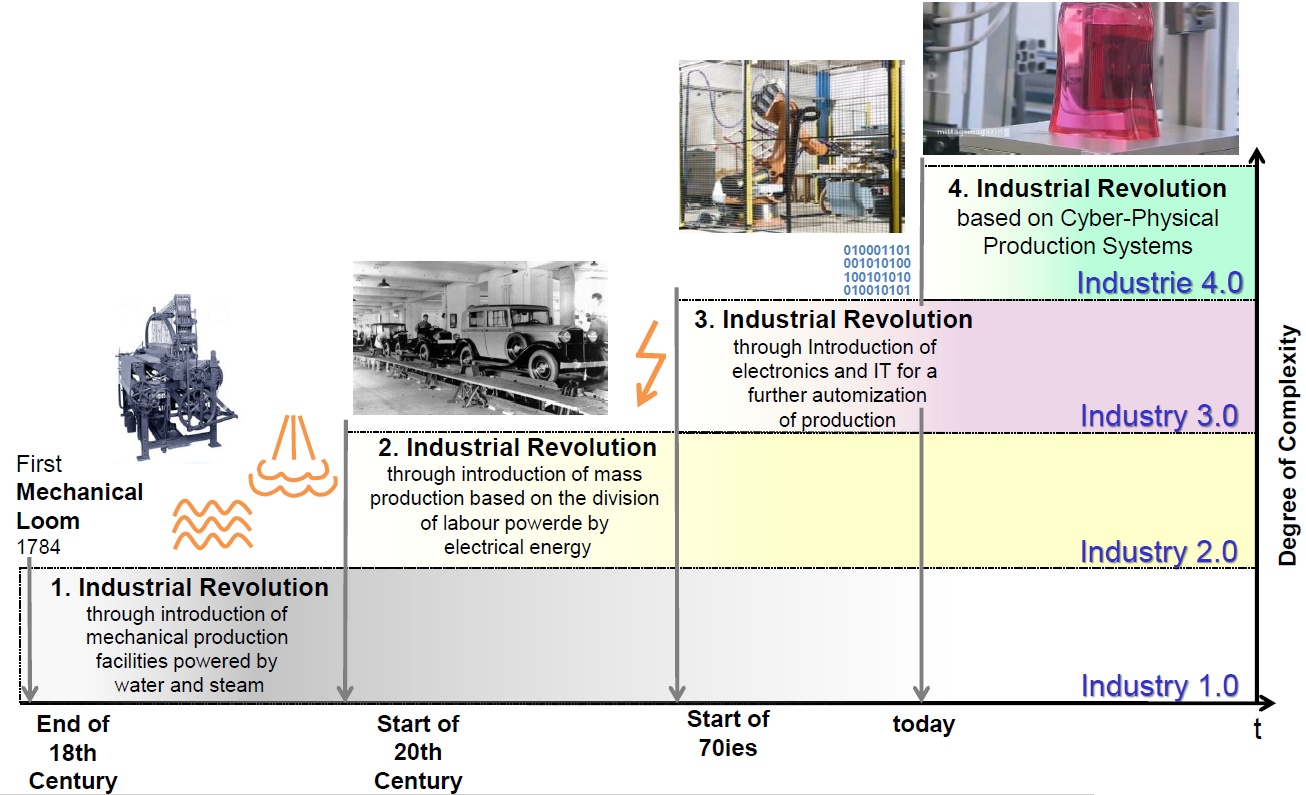
\includegraphics[width=1\textwidth]{i4-2.png}
		\fonte{\citeonline{wahlster2013industrie} (adaptado). }
	\end{figure}

	O termo I4.0 foi trazido a público pela primeira vez em 2011 na feira industrial de Hanôver (\textit{Hannover-Messe}) \cite{kagermann2011industrie}, que é uma feira tecnológica de grande relevância internacional e tem o costume de apresentar grandes inovações relacionadas ao setor industrial.

	Por vezes, a I4.0 é tratada também como a convergência da produção industrial com as novas Tecnologias de Informação e Comunicação (TIC) \cite{hermann2016design}.

	A quarta revolução industrial já está em curso segundo o Fórum Econômico Mundial \cite{schwab2016fourth} em seu encontro anual realizado em Davos no ano de 2016 e as razões para o surgimento deste novo paradigma de produção incluem: a competição acirrada entre empresas, alta complexidade de manufatura dos produtos e seus altos níveis de personalização por parte dos clientes \cite{bordeleau2018bi, vaidya2018industryfour}.

	Uma das bases para este novo paradigma de produção é a interligação de objetos no ambiente de produção por meio de identificadores individuais por meio dos conceitos de Internet das Coisas (\textit{Internet of Things} - IoT) e de Internet das Coisas Industrial (\textit{Industrial Internet of Things} - IIoT). Tais ``objetos'' se referem a equipamentos, produtos, máquinas, peças, pessoas e quaisquer outros elementos envolvidos no ambiente industrial, por vezes também são denominados ``ativos''.
	
	Esses ativos são inseridos no meio digital, onde podem trocar informações entre si e executarem comandos de funções sob seu respectivo correspondente físico de forma mais autônoma e com menor intervenção humana por meio do uso extensivo de recursos avançados de tecnologias da informação e comunicação \cite{adolph2018roadmap}. Devido a essa maior relação entre elementos do sistema de fabricação, extingui-se a relação essencialmente hierarquizada da indústria tradicional e os ativos passam a deter a capacidade de se comunicarem diretamente com outros elementos de diferentes níveis, conforme ilustrado na \autoref{fig:i3-to-i4}.
	
	\begin{figure}[htb]
		\centering
		\caption{Transição do (a) modelo hierárquico tradicional para o (b) modelo flexível de comunicação entre dispositivos na Indústria 4.0.}
		\label{fig:i3-to-i4}
		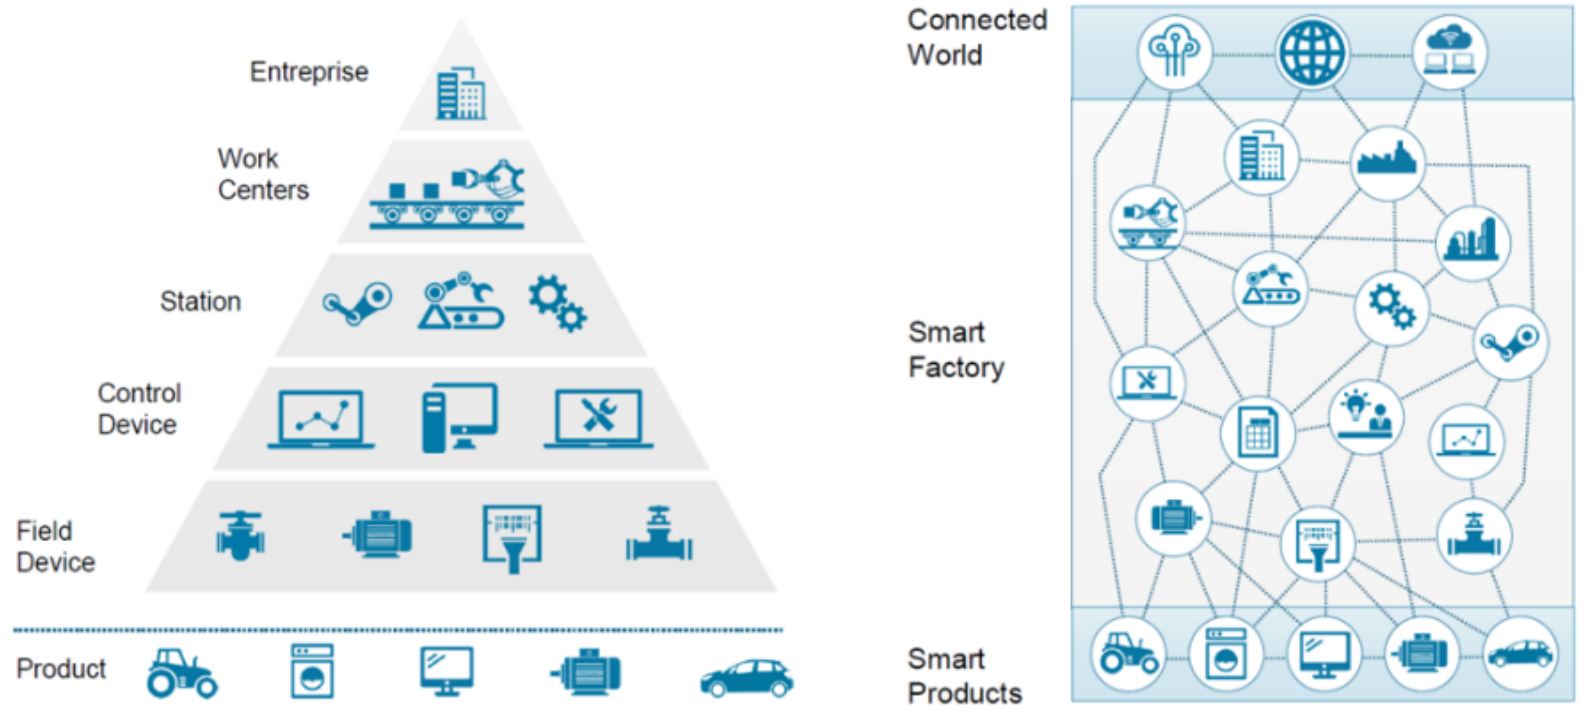
\includegraphics[width=1\textwidth]{i3-to-i4.png}
		\fonte{\citeonline{schmittner2017mtom} (adaptado).}
	\end{figure}

	Essa automatização e a troca de informações entre os ativos tem grande potencial de dar mais eficiência aos processos industriais, pois desta forma o sistema pode tomar decisões ótimas com base nas informações que lhe foram fornecidas por meio de sensores e identificadores. A visão para o futuro da produção baseado na I4.0 envolve sistemas de manufatura modulares e eficientes em cenários nos quais os produtos controlam seus próprios processos de fabricação \cite{lasi2014industryfour}.
	
	Há uma tendência global de redução do ciclo de vida do produto devida à rápida introdução de novas tecnologias para satisfazer a demanda dos clientes, especialmente em produtos eletrônicos \cite{trappey2008lifecycle}. A I4.0 beneficia a chegada de produtos com curto ciclo de vida uma vez que o produto controla seu próprio processo de fabricação, facilitando, assim, ajustes e personalização por parte do cliente, enquanto preserva os custos, a qualidade e o tempo de aprovisionamento (\textit{lead time}) da produção em massa.
	
	Indústria 4.0 é um conceito. Isto significa que são princípios a serem seguidos e implementados, porém o caminho para a implementação, assim como as tecnologias a serem adotadas podem ser diversas. As peculiaridades de cada indústria e de cada mercado estabelecem diferentes regras de negócios e, portanto, cada setor da indústria pode necessitar de diferentes formas e tecnologias para se implementar a I4.0 e se tornar uma fábrica inteligente. Alguns avanços tecnológicos, entretanto, são muito importantes ou essenciais para a implementação da I4.0 em qualquer sistema de manufatura, alguns deles são mostrados na \autoref{fig:tecnologias-i4}.
	
	\begin{figure}[htb]
		\centering
		\caption{Avanços tecnológicos que moldam a I4.0.}
		\label{fig:tecnologias-i4}
		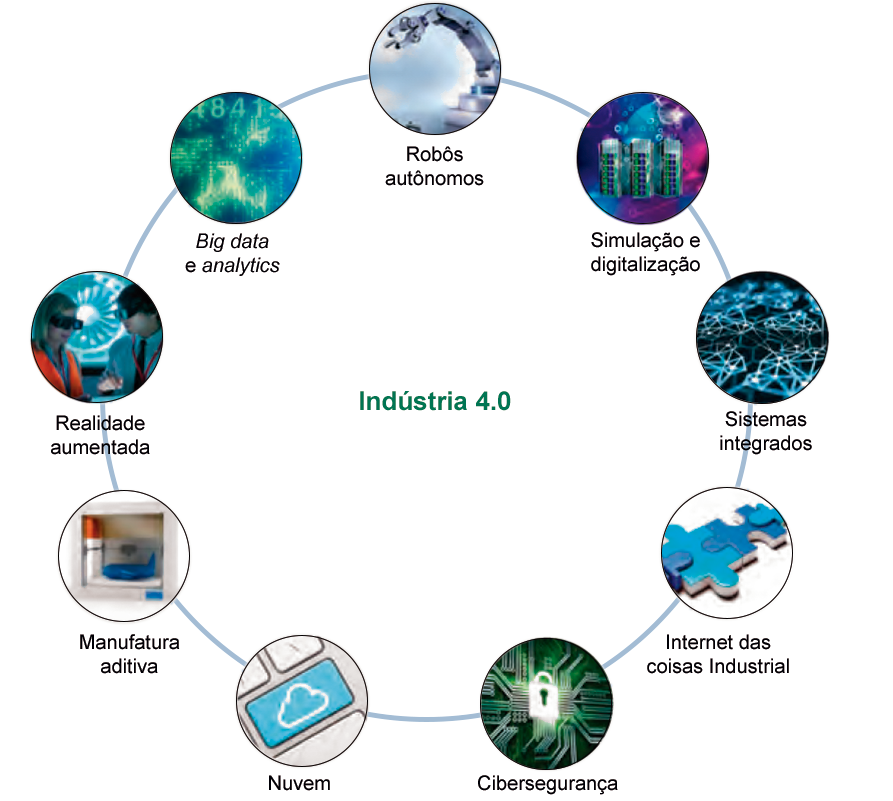
\includegraphics[width=0.9\textwidth]{tecnologias-i4.png}
		\fonte{\citeonline{russmann2015industryfour} (adaptado).}
	\end{figure}

	Após a primeira aparição do termo I4.0 na feira industrial de Hanôver em 2011, o termo ganhou significativa popularidade, principalmente no meio acadêmico e empresarial alemão. O termo foi então incentivado pelo governo alemão \cite{lasi2014industryfour, kagermann2013recommendations}, que apoiou a ideia e anunciou a Indústria 4.0 como parte integral de sua iniciativa estratégica para a indústria alemã, visando liderança em inovação tecnológica \cite{drath2014industrie} como uma abordagem para fortalecer a competitividade da indústria manufatureira alemã.	

	Por meio da iniciativa \textit{Plattform Industrie 4.0}, criada em 2013 pelo Ministério Federal da Educação e Pesquisa (\textit{Bundesministerium für Bildung und Forschung}) \cite{germany2019plattform} e com o grupo de trabalho ``Industrie 4.0 Working Group'' em comunicação com diversas associações de engenharia e indústrias alemãs, foram criados documentos oficiais como o ``\textit{Recommendations for implementing the strategic initiative Industrie 4.0}'' \cite{kagermann2013recommendations}, o ``\textit{German Standardization Roadmap - Industrie 4.0}'' \cite{adolph2018roadmap} e o ``\textit{Implementation Strategy Industrie 4.0}'' \cite{bitkom2016implementation} publicados em inglês com normas e diretrizes para a implementação da I4.0. Esta iniciativa atrelada ao entusiasmo acadêmico em torno do projeto I4.0 disseminaram o conceito fora da área de língua alemã e popularizou o termo I4.0 no mundo todo como epônimo de um futuro projeto no contexto de indústrias de alta tecnologia.

	O impacto econômico dessa revolução industrial será enorme, pois a I4.0 promete uma eficiência operacional substancialmente maior, bem como o surgimento de modelos de negócios, serviços e produtos de totalmente novos \cite{hermann2016design}.
	
	Em revoluções industriais passadas, os países pioneiros a se adaptarem às drásticas mudanças de produção foram os que mais se beneficiaram e se consolidaram como potências econômicas. Na quarta revolução industrial não será diferente. Embora a mudança completa para a I4.0 possa levar 20 anos para ser concretizada \cite{russmann2015industryfour}, nos próximos anos serão estabelecidos avanços importantes que definirão os pioneiros e detentores de tecnologias dessa nova revolução. Portanto, é de interesse de cada país liderar a concorrência global por meio de sua consolidação como mercado líder e fornecedor de soluções para a Indústria 4.0.

	\subsection{Modelo de Arquitetura de Referência para a Indústria 4.0}
	
	O Modelo de Arquitetura de Referência para a Indústria 4.0, abreviado RAMI4.0, consiste em um sistema de coordenadas tridimensional que descreve todos os aspectos cruciais da Indústria 4.0. Dessa maneira, inter-relações complexas podem ser divididas em grupos menores e mais simples.
	
	A \autoref{fig:rami4} mostra a representação do RAMI4.0 e especifica os itens contidos em cada eixo. A \autoref{tab:rami-eixos} fornece uma breve descrição de cada eixo do RAMI4.0.
	
	\begin{table}[htb]
		\centering
		\footnotesize
		\caption{Eixos do RAMI4.0}
		\label{tab:rami-eixos}
		\begin{tabular}{p{3cm}p{12cm}}
			\hline
			\textbf{Eixo} &\textbf{Descrição} \\
			
			\hline
			Camadas
			& As seis camadas no eixo vertical descrevem a decomposição de um ativo em suas funcionalidades, isto é, o mapeamento virtual de um ativo. A representação em camadas se origina da tecnologia da informação e comunicação (TIC), onde as funcionalidades de sistemas complexos são comumente divididas em camadas. \\
			
			
			\hline
			Ciclo de vida e  Cadeia de valor
			& O eixo horizontal esquerdo representa o ciclo de vida das instalações e produtos, com base na IEC 62890 para gerenciamento do ciclo de vida. Além disso, é feita uma distinção entre ``tipos'' e ``instâncias''. Um ``tipo' é criado na fase de desenvolvimento e, uma vez concluída esta fase, este tipo é liberado para a produção, servindo como modelo para uma ``instância'', que é quando produto real está sendo fabricado e possui um número de série. \\
			
			\hline
			Níveis hierárquicos
			& No eixo horizontal direito estão indicados os níveis hierárquicos da IEC 62264, a série de padrões internacionais para sistemas de TI e controle corporativos. Os níveis hierárquicos representam as diferentes funcionalidades das fábricas. Para representar o ambiente I4.0, as funcionalidades foram expandidas, incluindo assim o ``Produto'', o ``Dispositivo de campo'' e a conexão com a IoT (Mundo conectado). \\
			\hline
			
		\end{tabular}
		\fonte{O autor.}
	\end{table}

	A \autoref{fig:eixo-camadas} mostra o detalhamento de cada elemento do eixo Camadas do RAMI4.0 e sua associação ao modelo completo.
	
	\begin{figure}[htb]
		\centering
		\caption{(a) Detalhamento de cada elemento do Eixo Camadas e (b) representação completa do RAMI4.0.}
		\label{fig:eixo-camadas}
		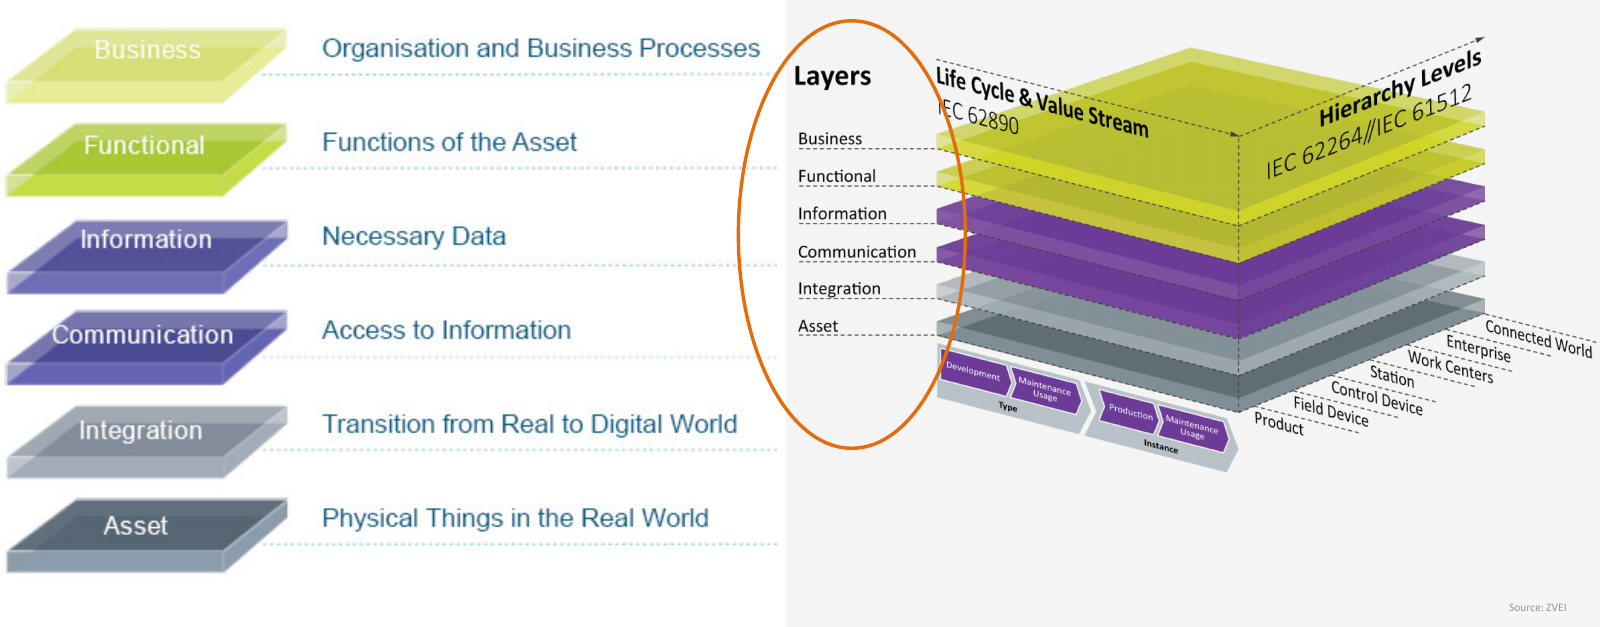
\includegraphics[width=1\textwidth]{eixo-camadas.png}
		\fonte{\citeonline{gayko2018ramistandardization} (adaptado).}
	\end{figure}

	São 6 as camadas do RAMI4.0. O propósito de cada camada, começando da mais inferior (Ativo) para a mais elevada (Regra de Negócio), é descrito a seguir \cite{bitkom2016implementation}:
	
	\begin{enumerate}
		\item \textbf{Ativo}: Representa um elemento da realidade e não necessariamente físico, como, por exemplo, um máquina, um \textit{software}, uma documentação, uma ideia, etc. O trabalhador e seu conhecimento sendo aplicado representa também um ativo. Os ativos são integrados ao meio digital através da camada de Integração.
		
		\item \textbf{Integração}: Camada responsável pela extração e fornecimento de informações sobre os ativos para as camadas superiores. Representa a digitalização dos ativos. Cada evento no mundo real é refletido também em um evento no mundo virtual. Se a realidade mudar, este evento então é relatado à camada de integração e os dados são atualizados no mundo virtual.
		
		\item \textbf{Comunicação}: Padronização da comunicação por meio da adoção de um formato de troca de dados uniforme entre os dispositivos. Esta camada é a responsável pela interoperabilidade entre os ativos na I4.0. A camada de Comunicação fornece dados sobre o ativo à camada de informação.
		
		\item \textbf{Informação}: Controle dos dados do ativo. Esta camada agrega todos dados sobre um determinado ativo e é responsável pelo gerenciamento destes dados. Na camada de informação são garantidos que os dados sejam tratados, pré-processados, armazenados e disponibilizados para os demais ativos na rede.
		
		\item \textbf{Funcional}: Contém a descrição formal de todas as funcionalidades do sistema. É também a plataforma para integração horizontal das funcionalidades. As regras de negócio e a lógica de tomada de decisão são geradas dentro desta camada. A camada funcional é a interface para fornecimento de informações por meio de microsserviços para outros ativos tanto dentro (integração vertical) como fora (integração horizontal) da empresa.
			
		\item \textbf{Regra de negócio}: Contêm as regras de negócio que o sistema deve seguir como, por exemplo, as condições legais e regulatórias. A camada Regra de negócio também é responsável por mapear os modelos de negócios do sistema e orquestrar os serviços da camada funcional.
	\end{enumerate}

	Já os elementos do eixo ``Ciclo de Vida e Cadeia de Valor'' do RAMI4.0 são detalhados na \autoref{fig:eixo-ciclodevida}, juntamente com seu destaque dentro do modelo completo.
	
	\begin{figure}[htb]
		\centering
		\caption{(a) Detalhamento do eixo Ciclo de Vida e Cadeia de Valor e (b) representação completa do RAMI4.0.}
		\label{fig:eixo-ciclodevida}
		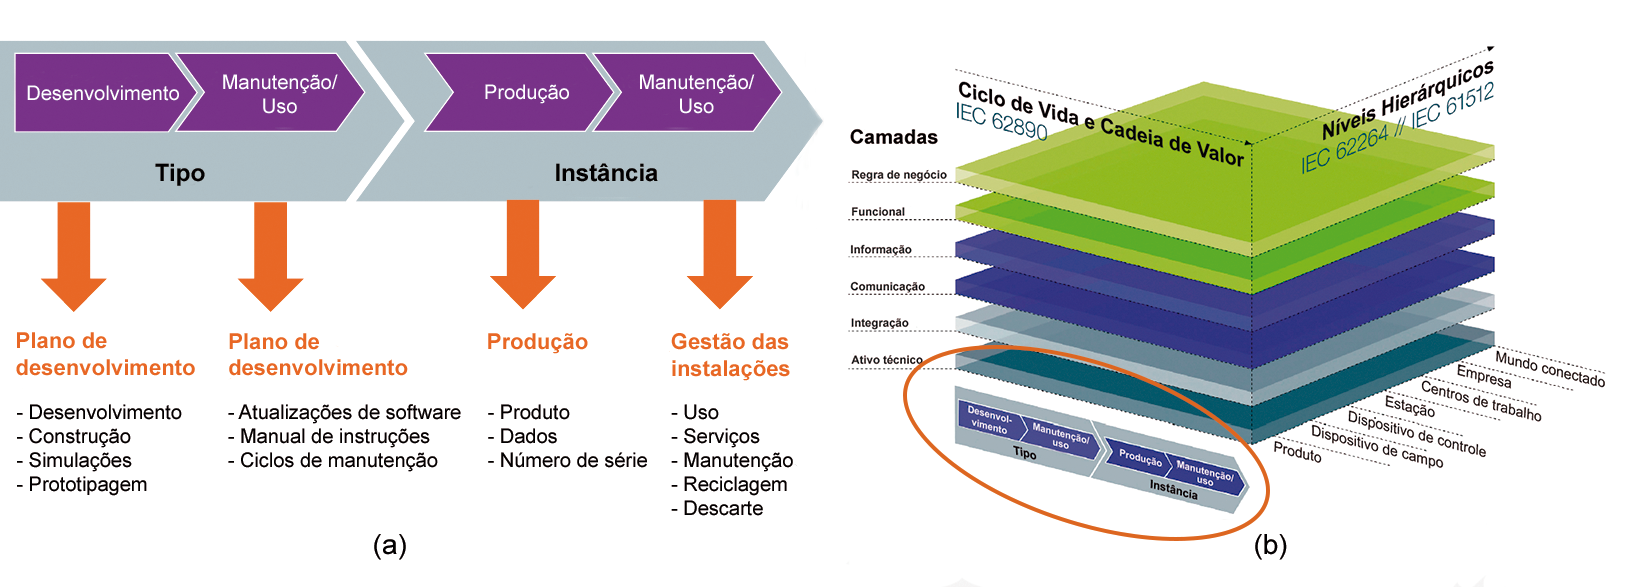
\includegraphics[width=1\textwidth]{eixo-ciclodevida.png}
		\fonte{\citeonline{gayko2018ramistandardization} (adaptado).}
	\end{figure}

	A I4.0 oferece um grande potencial de aprimoramento dos processos ao longo do ciclo de vida do produto. O eixo Ciclo de vida e Cadeia de valor fornece uma representação do estado do ativo ao longo de toda a cadeia de suprimentos correspondente a sua cadeia de valor. 
	
	É feita a distinção fundamental entre ``tipo'' e ``instância'', cada um correspondendo a uma fase em que o produto se encontra \cite{adolphs2015rami}.
	
	Um \textbf{tipo} é sempre criado com uma ideia inicial, ou seja, quando um produto surge na fase de desenvolvimento. Isso abrange o comissionamento, desenvolvimento e testes até a produção inicial de amostras e protótipos. \cite{adolph2018roadmap}. 
	
	Com a conclusão de todas as etapas de testes e validação, o tipo é liberado para produção em série. A partir de então, novos produtos podem ser instanciados com base neste ``tipo'' validado. 
	
	Com a fabricação do produto, \textbf{instâncias} são geradas. Cada produto fabricado representa uma instância de um determinado tipo e recebe um número de série exclusivo.
	
	As melhorias sobre um produto feitas pelo fabricante refletem em um novo ``tipo'', que por sua vez pode ser usado para fabricar novas instâncias, acompanhando, assim, o ciclo de vida do produto.

	Finalmente o eixo ``Níveis Hierárquicos'' do RAMI4.0 é apresentado na \autoref{fig:eixo-niveishierarquicos}.
	
	\begin{figure}[htb]
		\centering
		\caption{(a) Detalhamento do eixo Níveis Hierárquicos do RAMI4.0 e (b) representação completa do RAMI4.0.}
		\label{fig:eixo-niveishierarquicos}
		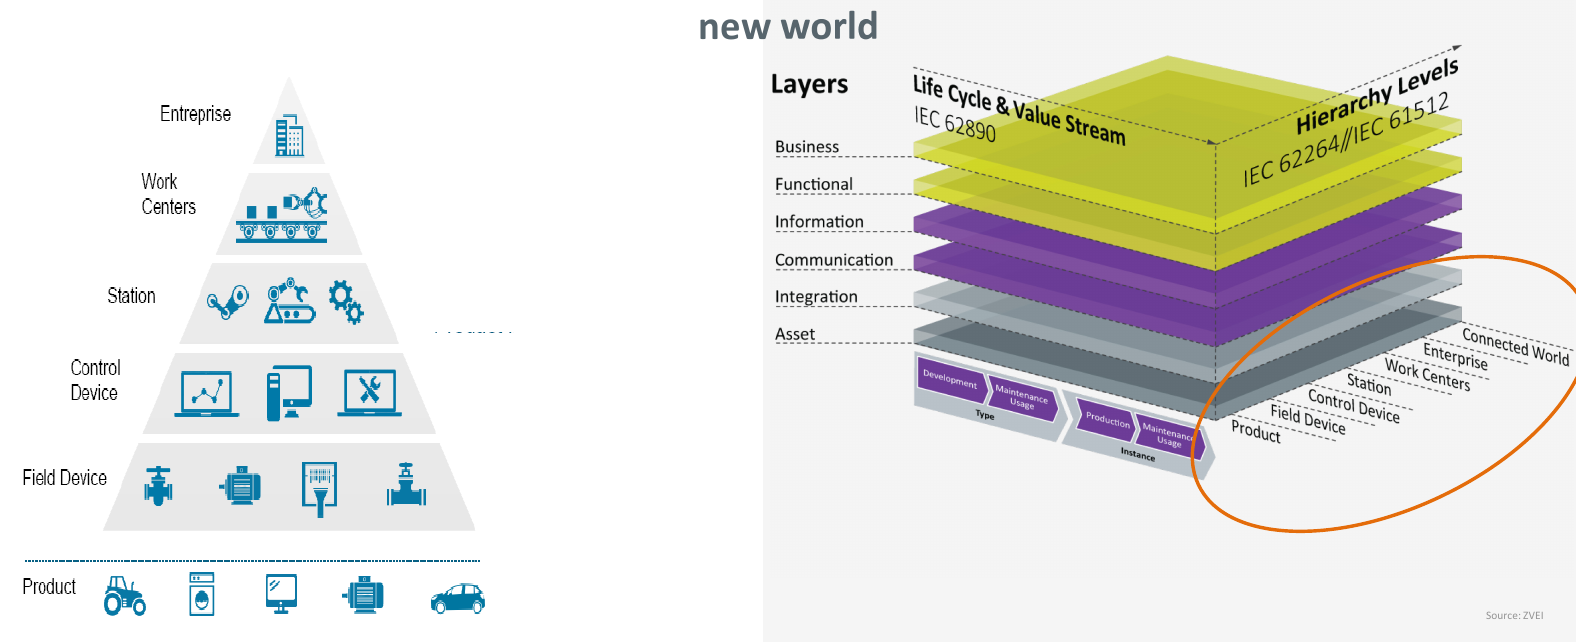
\includegraphics[width=1\textwidth]{eixo-niveishierarquicos.png}
		\fonte{\citeonline{gayko2018ramistandardization} (adaptado).}
	\end{figure}

	O eixo Níveis Hierárquicos do RAMI 4.0 descreve a integração dos sistemas empresariais de controle \cite{pisching2018arquitetura}. Este eixo representa as diferentes funcionalidades das fábricas.
	
	É uma reformulação da norma ISA-95 para o contexto da I4.0 e define a classificação funcional de cada ativo da Indústria 4.0, direcionando as etapas da produção para as demais funções. Os níveis hierárquicos do RAMI 4.0 são divididos em \cite{adolphs2015rami}:
	 
	\begin{itemize}
			\item Produto;
			\item Dispositivo de campo;
			\item Dispositivo de controle;
			\item Estação de trabalho;
			\item Centros de trabalho;
			\item Empresa;
			\item Mundo conectado.
	\end{itemize}
	
	Dentro dos três eixos, todos os aspectos cruciais da I4.0 podem ser mapeados, permitindo que os ativos sejam classificados devidamente de acordo com o modelo. Os conceitos altamente flexíveis da I4.0 podem, assim, ser descritos e implementados usando o RAMI4.0. O modelo de arquitetura de referência permite a migração passo a passo do presente estado da indústria para o mundo da Indústria 4.0.
	
	\subsection{Asset Administration Shell}
	
	Um ativo é qualquer coisa que precise ser conectada para agregar valor a um processo industrial \cite{bader2019aas}, ou seja, todos os itens que têm valor em um caso de uso específico. Na I4.0, isso pode ser um produto físico, uma peça de equipamento, um \textit{Software} ou documentos como plantas, contratos, pedidos, etc.
	
	No paradigma da I4.0, cada ativo é encapsulado por uma camada (ou casca) de administração, também chamada de \textit{Administration Shell}. O \textit{Administration Shell} do ativo técnico é denominado ``\textit{Asset Administration Shell}'' (AAS). Este AAS é a representação da parte virtual/digital de um ativo no mundo I4.0 \cite{ye2019aas}.
	
	Fazendo uma associação ao RAMI4.0, o AAS engloba as camadas digitais, sendo elas: Comunicação, Informação, Funcional e Regra de Negócio; parte da camada Integração também é contemplada pelo AAS, já que essa é a conexão entre o ativo e o meio virtual. Tal associação é representada pela \autoref{fig:aas-rami}.

	\begin{figure}[htb]
		\centering
		\caption{Representação do AAS como a parte virtual do Componente I4.0.}
		\label{fig:aas-rami}
		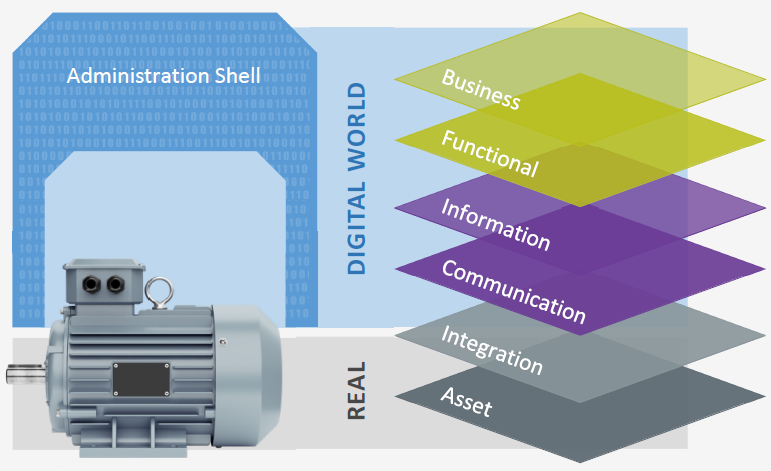
\includegraphics[width=0.8\textwidth]{aas-rami.png}
		\fonte{\citeonline{gayko2018ramistandardization} (adaptado).}
	\end{figure}
		
	O AAS consiste em vários submodelos nos quais são descritos todas as informações e funcionalidades de um determinado ativo, incluindo suas características, propriedades, condição, parâmetros, dados de medições e capacidades \cite{bader2019aas}. A \autoref{fig:aas-submodelos} exemplifica um AAS como sendo uma ``casca'' que engloba o ativo em si, essa casca contém informações relevantes do ativo em forma de ``submodelos''.
	
	\begin{figure}[htb]
		\centering
		\caption{Exemplificação de um AAS para um servomotor, incluindo os submodelos de dados técnicos, dados operacionais e documentação.}
		\label{fig:aas-submodelos}
		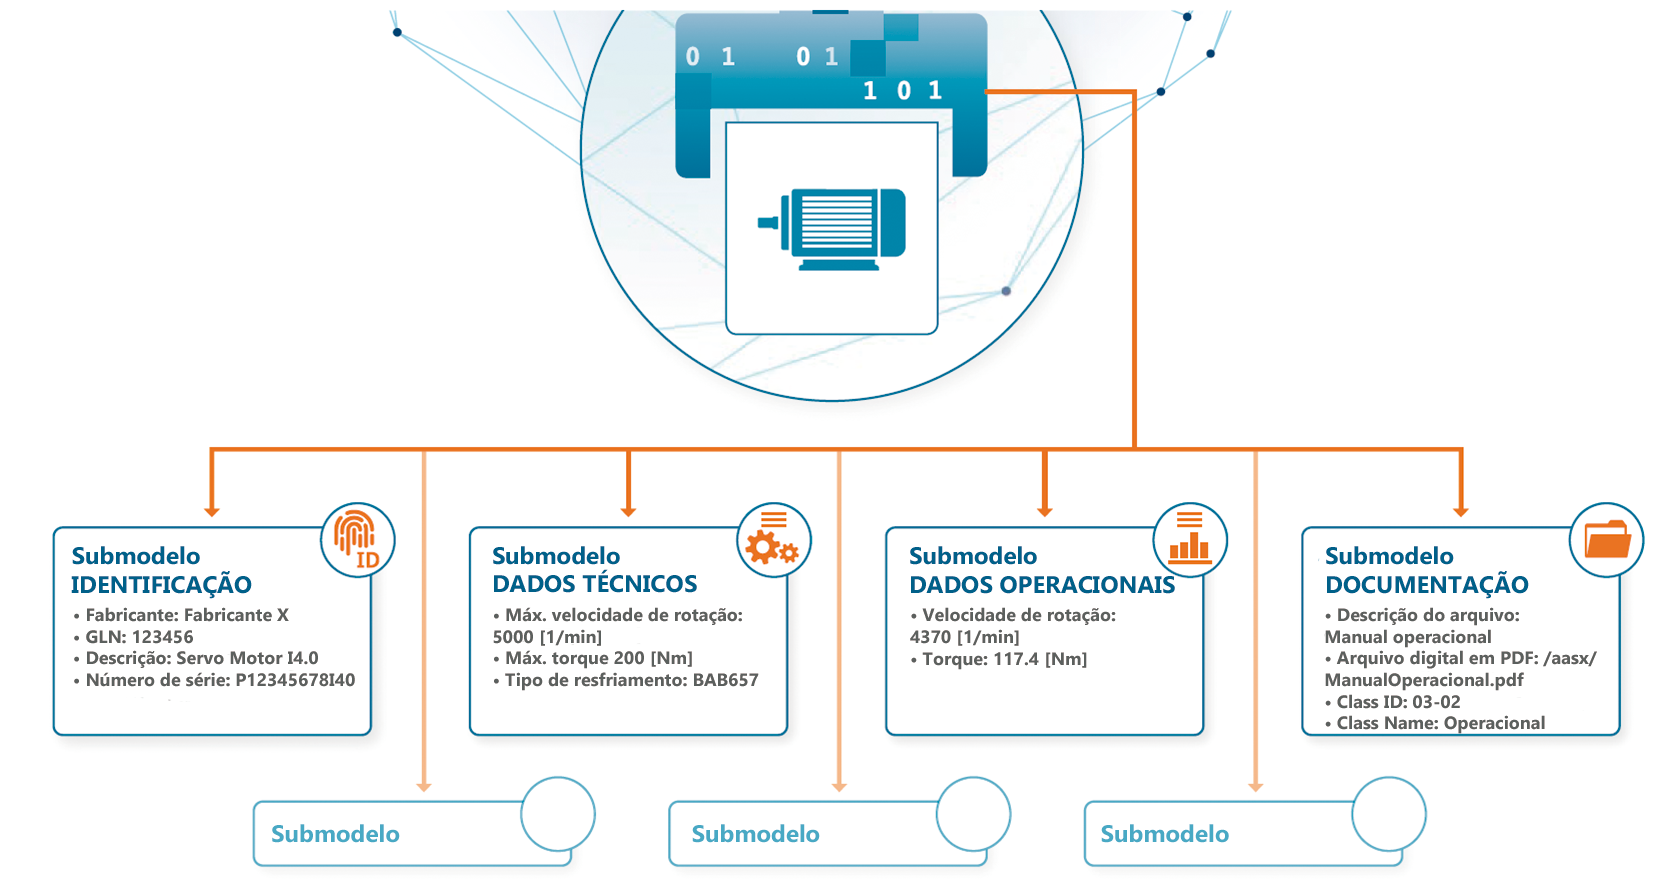
\includegraphics[width=1\textwidth]{aas-submodelos.png}
		\fonte{\citeonline{bader2019aas} (adaptado).}
	\end{figure}

	Os submodelos são unidades básicas de organização dentro de um AAS que agregam informações semelhantes. Eles são divididos em dois tipos \cite{plattform2019detailsaas}: submodelos básicos e submodelos livres \cite{bader2019aas}.
	
	Os submodelos básicos são unidades de organização que se aplicam a muitos ou todos os ativos dentro do mundo I4.0. Já os submodelos livre são acertados entre os parceiros na cadeia de suprimentos e possuem um uso específico para um determinado produto.
	
	O AAS é um elo entre os ativos reais e seus correspondentes digitais no mundo conectado. A \autoref{fig:aas-conexao} ilustra a comunicação entre diferentes AASs em um ambiente de manufatura I4.0 sob uma ontologia comum.
	
	\begin{figure}[htb]
		\centering
		\caption{Comunicação entre AASs de componentes I4.0.}
		\label{fig:aas-conexao}
		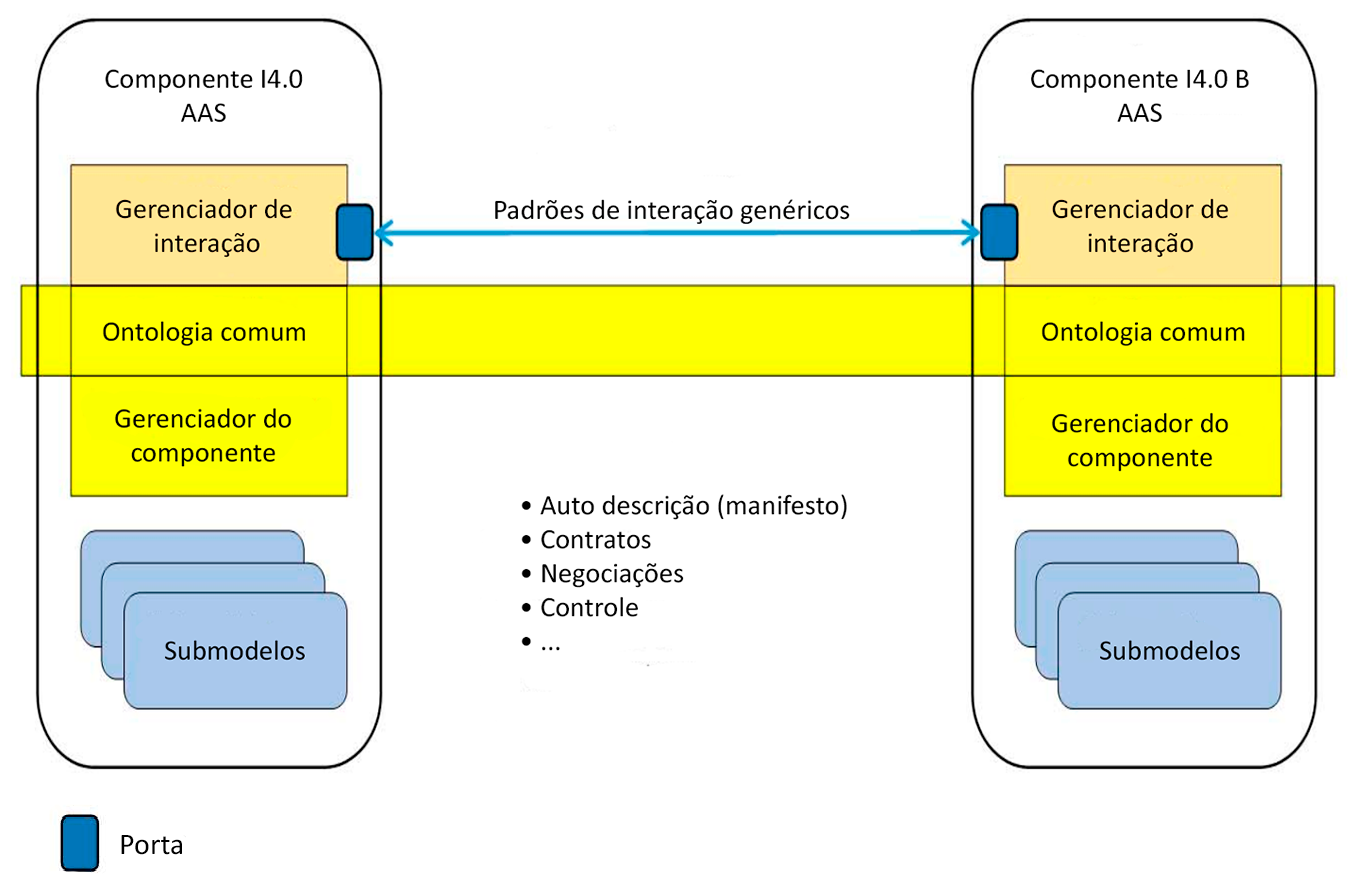
\includegraphics[width=1\textwidth]{aas-conexao.png}
		\fonte{\citeonline{marcon2018asset} (adaptado).}
	\end{figure}

	Dentro da I4.0, todos os ativos possuem um AAS com capacidade de comunicação com outros dispositivos. O conjunto Ativo-AAS, que é o objeto real encapsulado pelo \textit{Asset Administration Shell}, é denominado ``Componente I4.0''.
	
	A integração dos ativos, representada pelos Componentes I4.0, em um nível funcional requer uma descrição padronizada das funções (ou capacidades) dos ativos em questão. A padronização de submodelos para descrever detalhadamente cada função pode ser usada para definir requisitos para a fabricação de produtos \cite{bedenbender2017aasexamples}. A \autoref{fig:submodelos} mostra um exemplo de detalhamento de funções sobre um ativo.
	
	\begin{figure}[htb]
		\centering
		\caption{Detalhamento de funções no AAS por meio de submodelos.}
		\label{fig:submodelos}
		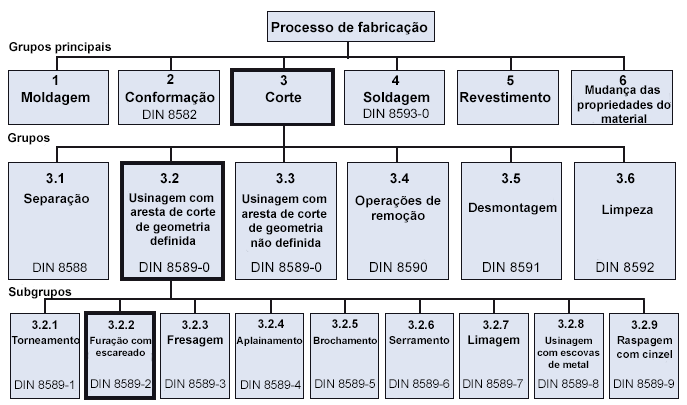
\includegraphics[width=1\textwidth]{submodelos.png}
		\fonte{\citeonline{bedenbender2017aasexamples} (adaptado).}
	\end{figure}

	No ambiente de manufatura baseado na I4.0, o produto descreve os requerimentos necessários para sua fabricação e então esses requerimentos são comparados com as descrições da funções das máquinas disponíveis. Portanto, a seleção de um ativo é otimizada, baseando-se nos requerimentos do produto e nas descrições das funções dos ativos.

\section{Memória digital do produto}

	Os produtos que são produzidos no cenário de Indústria 4.0 são equipados com a mémoria digital do produto (MDP). Por meio dessa memória podem ser acessadas e redistribuídas informações sobre o produto ao longo de toda a cadeia de valores.

	A MDP é alimentada e disponibilizada ao longo de todo o ciclo de vida do produto, podendo ser acessada por qualquer elo na cadeia de suprimentos (fabricante, distribuidor, varejista, consumidor). Mesmo no pós-venda, a MDP ainda se faz presente. O consumidor ainda pode ter acesso às informações dos produtos em cada ponto da cadeia de suprimentos e se beneficiar de serviços individuais que se acumulam na memória \cite{brandherm2011productmemory}.

	Nesse contexto, a MDP mantém informações relevantes de eventos ocorridos ao longo do ciclo de vida do produto a fim de fornecer serviços a todo o ambiente com o qual o produto se relaciona \cite{brandherm2011productmemory}.
	
	A MDP fornece também uma forma de rastreabilidade de produtos ao longo da cadeia de valores uma vez que pode armazenar informações geoespaciais do ativo ao longo do tempo.

\section{Arquitetura orientada a serviços (SOA)}
	
	Arquitetura Orientada a Serviços (SOA) é um estilo de projeto de software em que serviços são disponibilizados a outros sistemas por meio de protocolo de comunicação comum em uma rede \cite{bell2008soa}. Um serviço SOA é uma unidade de funcionalidade que pode ser fornecida/acessada remotamente. A SOA se destina a ser independente de fornecedores, produtos e tecnologias.
	
	Para quem consome um serviço SOA, a abordagem é como uma caixa preta, o que significa que o consumidor não não sabe ou não precisa estar ciente do funcionamento interno do serviço, sendo apenas o resultado do serviço relevante. Os serviços SOA representam uma lógica de fornecimento de resultados que possibilitam a abstração de problemas.
	
	Dentro do mundo da Indústria 4.0 e de sistemas produtivo, a SOA é uma abordagem que	traz novas perspectivas uma vez que se estabelece um conjunto de princípios para uma arquitetura de sistema autônomo e interoperável \cite{candido2009soa}, que tem por objetivo aumentar a eficiência, agilidade e produtividade de um sistema por meio da adoção generalizada do conceito de serviços. \cite{souit2013soa}.
	
	Os serviços SOA dentro do ambiente de manufatura encapsulam as funcionalidades necessárias, ocultando todas as heterogeneidades das partes do sistema, permitindo, desta forma, características de flexibilidade, confiabilidade e fácil implementação de	soluções \cite{groba2008soa}.
	
	A SOA dentro do meio industrial permite que um sistema atue como \textit{Middleware}, ou seja, uma camada ou componente de software que integra os diferentes aplicativos em um sistema. A \autoref{fig:middleware} ilustra como se dá a interconexão entre os elementos do sistema com e sem um \textit{middleware}.
	
	\begin{figure}[htb]
		\centering
		\caption{Interconexão entre os elementos do sistema com e sem um \textit{middleware}.}
		\label{fig:middleware}
		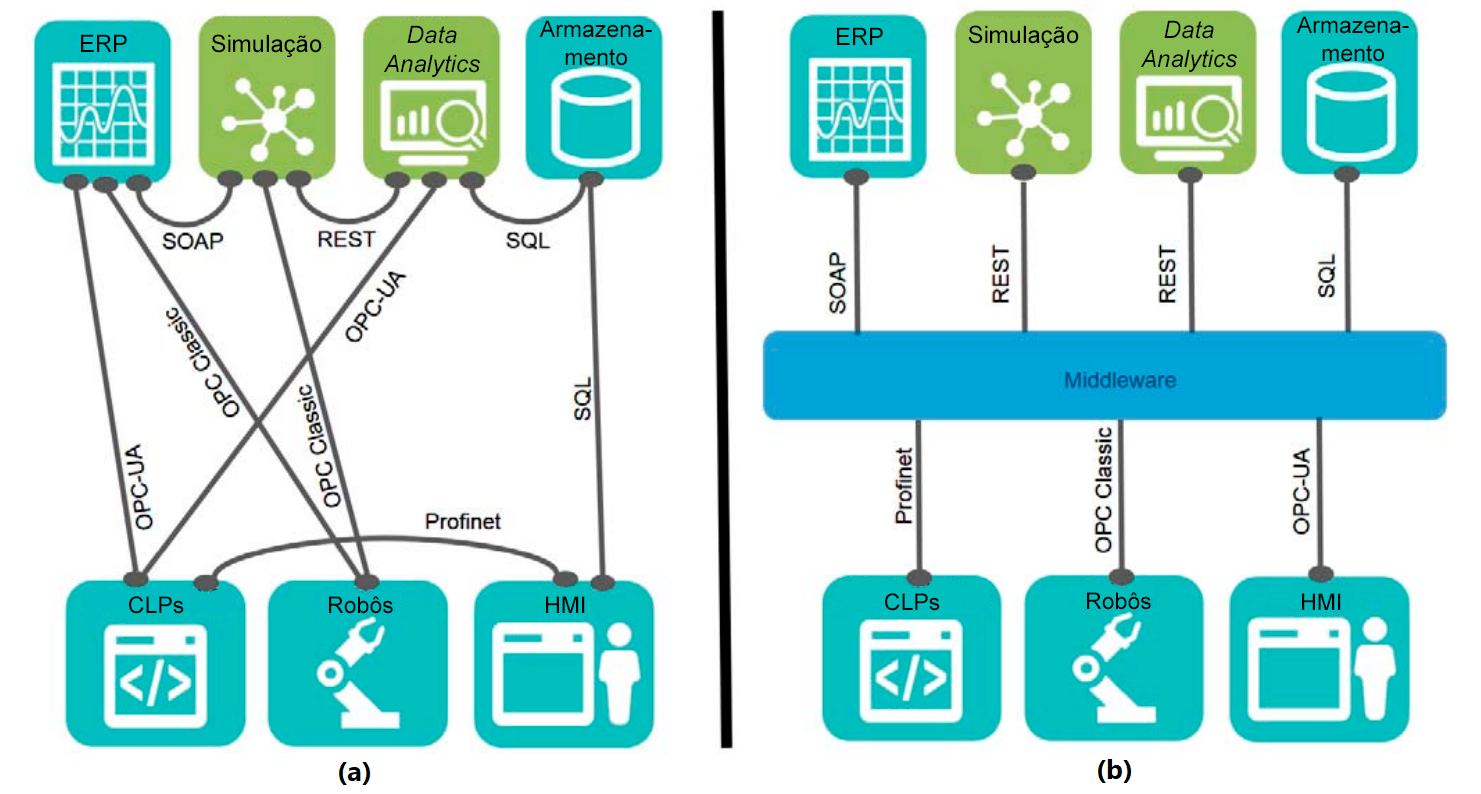
\includegraphics[width=0.9\textwidth]{middleware.png}
		\fonte{\citeonline{gosewehr2017middleware} (adaptado).}
	\end{figure}

	SOA está relacionado à ideia de uma Interface de Programação de Aplicação (Application Programming Interface - API), que é o conjunto de rotinas e padrões estabelecidos por um \textit{software} para a utilização das suas funcionalidades por aplicativos externos.
	
	Para se disponibilizar um serviço SOA, os Web Services (WSs) são a tecnologia mais adotada para
	implementar uma API \cite{souit2013soa}. Os WSs podem ser vistos como uma tecnologia padrão para facilitar a interoperabilidade, integração e reuso de componentes da aplicação, isto é, serviços.
	
	\subsection{Serviços Web}
	
	Um serviço da Web é uma interface que descreve uma série de operações acessíveis por meio de uma linguagem de descrição de serviços padronizada \cite{gottschalk2002webservices}. Um serviço da Web executa uma tarefa específica ou um conjunto de tarefas e retorna ao usuário o resultado da operação. Cada aplicação pode ter a sua própria linguagem, que é traduzida para uma linguagem comum, como um XML, JSON, CSV, etc.
	
	Por meio de WSs, as aplicações podem ser descritas, publicadas, localizadas e invocadas em uma rede de comunicação tipo www (World Wide Web) \cite{souit2013soa}.
	
	A arquitetura do Web Service é constituída por três atores básicos: o provedor, o repositório e o solicitante; e por três operações básicas: a publicação, a procura e a interação \cite{gottschalk2002webservices}. A \autoref{fig:componentes-webservice} ilustra os atores e a interação entre eles por meio das operações.
	
	Detalhadamente, os atores em um WS são:
	
	\begin{itemize}
		\item \textbf{Provedor de serviços}: Representa a plataforma que hospeda e fornece um determinado serviço, esta plataforma permite que clientes solicitem serviços e recebam suas respectivas respostas. O provedor de serviços é responsável também por fornecer uma descrição sobre o serviço prestado e publicar esta descrição em um repositório acessível pelo solicitante.
		
		\item \textbf{Repositório}: É uma plataforma acessível com a função de armazenar e fornecer a descrição sobre diversos WSs. Os WSs são descobertos pelo solicitante por meio do repositório para que assim possa decidir o serviço que melhor o atenda.
		
		\item \textbf{Solicitante de serviços}: É o ator que necessita de um determinado serviço e requisita a sua execução. O solicitante de serviço pode ser uma pessoa acessando um navegador ou uma aplicação realizando solicitações por meio de APIs.		
	\end{itemize}

	\begin{figure}[htb]
		\centering
		\caption{Componentes de um WS e operações.}
		\label{fig:componentes-webservice}
		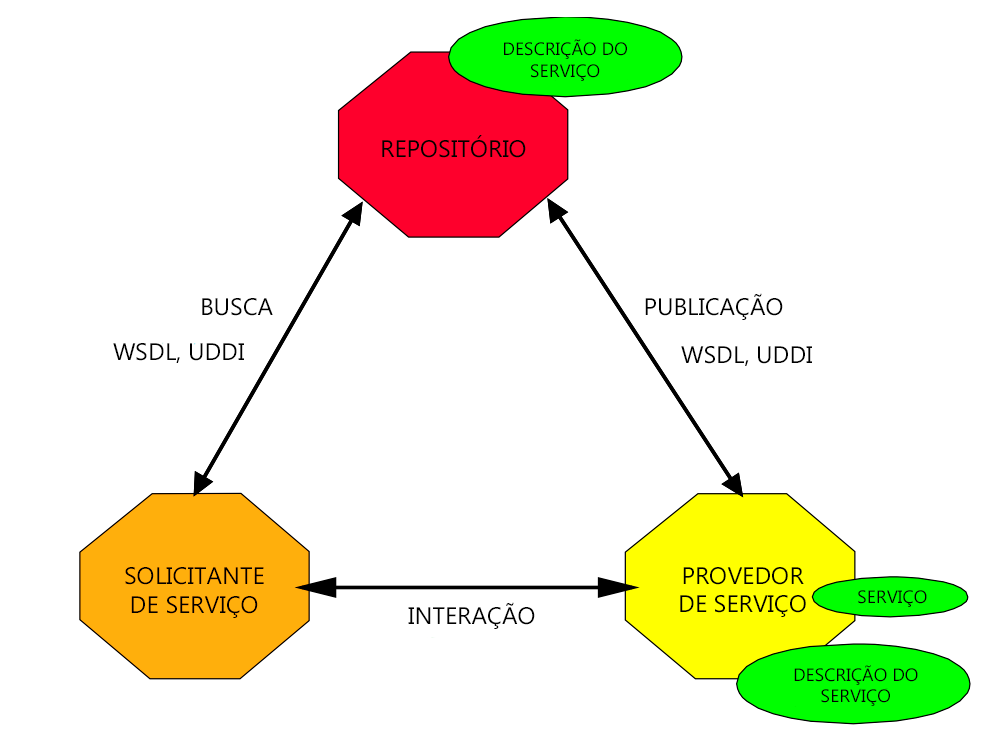
\includegraphics[width=0.8\textwidth]{componentes-webservice}
		\fonte{\citeonline{kreger2001webservices} (adaptado).}
	\end{figure}
	
	Já as operações básicas em WS em detalhe são:
	
	\begin{itemize}
		\item \textbf{Publicação}: Publicação pelo provedor da descrição do serviço em um repositório para que o serviço se torne acessível a público e solicitantes possam localizá-lo. 
		\item \textbf{Busca}: Busca e recebimento da descrição de um serviço. O solicitante pode receber a descrição do serviço pelo provedor ou por meio do repositório.
		\item \textbf{Interação}: Comunicação direta entre solicitante e provedor para o fornecimento de serviços. Nesta fase, o solicitante se decide por um determinado serviço dentro os disponíveis no repositório e inicia uma interação com o provedor por meio de uma API.
	\end{itemize}
	
	As etapas de interação entre as entidades são representadas por meio de diagrama UML na \autoref{fig:uml-webservice}.
	
	\begin{figure}[htb]
		\centering
		\caption{Diagrama UML com os atores e interações em um WS.}
		\label{fig:uml-webservice}
		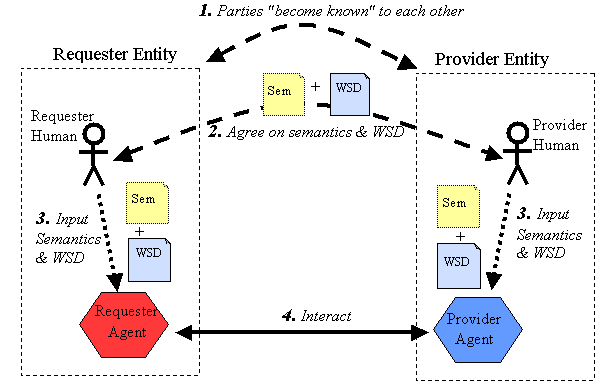
\includegraphics[width=1\textwidth]{uml-webservice}
		\fonte{\citeonline{booth2004webservice} (adaptado).}
	\end{figure}

	Os WSs se tornaram bastante atrativos, pois este modelo pode ser aplicado com tecnologias acessíveis ao solicitante, em particular XML e HTTP, que podem ser acessadas pela maioria dos navegadores convencionais. A disponibilização de serviços interativos na Web se tornou muito popular e com isso aparecem novos modelos de negócios como o SaaS (\textit{Software as a Service}), PaaS (\textit{Platform as a Service}), IaaS (\textit{Infrastructure as a Service}), etc.
	
	Dentro do mundo da Indústria 4.0 não é diferente. Ativos podem publicar suas funcionalidades em repositórios e executarem determinadas tarefas mediante solicitação por parte do solicitante, podendo assim serem classificados uma manufatura como um serviço (\textit{Manufacturing as a Service}) \cite{annunziata2019maas, nichols2020maas, siepen2019maas}.
	
	\subsection{Transferência Representacional de Estado}
	
	A Transferência Representacional de Estado (\textit{Representational State Transfer} - REST) é uma arquitetura de \textit{software} que define padrões para acesso e disponibilização de \textit{Web Services} (WSs). Os WSs que seguem o padrão REST são denominados \textit{RESTful Services}.
	
	A arquitetura REST possibilidade a interoperabilidade entre sistemas na Internet, pois permitem que os sistemas solicitantes acessem e manipulem representações textuais de recursos usando um conjunto uniforme e predefinido de operações sem estado \cite{ferris2004webservices}.
	
	Quando o HTTP é usado como protocolo de comunicação em um serviço REST, cada método do protocolo recebe um tipo de operação padrão do REST. A \autoref{tab:rest} mostra as possíveis operações em um RESTful Service e seu método HTTP correspondente, quando este protocolo é utilizado.
	

	\begin{table}[htb]
		\centering
		\footnotesize
		\caption{Possíveis operações em um \textit{RESTful Service}.}
		\label{tab:rest}
		\begin{tabular}{p{2cm}p{2cm}p{8cm}}
			\hline
			\textbf{Operação} &
			\textbf{Método \newline HTTP} &
			\textbf{Resposta} \\[5mm]

			\hline
			Criação &
			POST &
			201 (Criado) \\[5mm]
			
			\hline
			Leitura &
			GET &
			200 (OK), 404 (Não encontrado)  \\[5mm]
			
			\hline
			Atualização &
			PATCH &
			200 (OK), 204 (Sem conteúdo), 404 (Não encontrado),405 (Não permitido) \\[5mm]
			
			
			\hline
			Exclusão &
			DELETE &
			200 (OK), 404 (Não encontrado), 405 (Não permitido) \\[5mm]
			
			\hline
		\end{tabular}
		\fonte{\cite{fielding2000architecture} (adaptado).}
	\end{table}
